%optics
In this part the  some theorems from the geometric optics  are introduced as the basic knowledges.

\subsection{Lens Optics}
Lens is widely applied in optics. Some are used for photography of camera; some are used for microscopes and telescopes.  In this work lens is used for coupling fibers to photonic waveguide. No matter what kind of application they all base on primary rules: lens theory.\\
One important function of lens is focus. It is a common experience by using a magnifying glass to set small pieces of paper or leaves on fire with sunlight. In this scene the lens of the magnifying glass focuses all incoming sun rays at a single spot. This spot is called focal point and the distance between the focal point and the center of the lens is called focal length $f$. The dimensions of this spot and the focal length are two primary characters of the lens and values of them depend on the radius of curvature of the lens surface and on the refractive index of the material the lens is made from. \\
\begin{figure}[httbp]
\centering
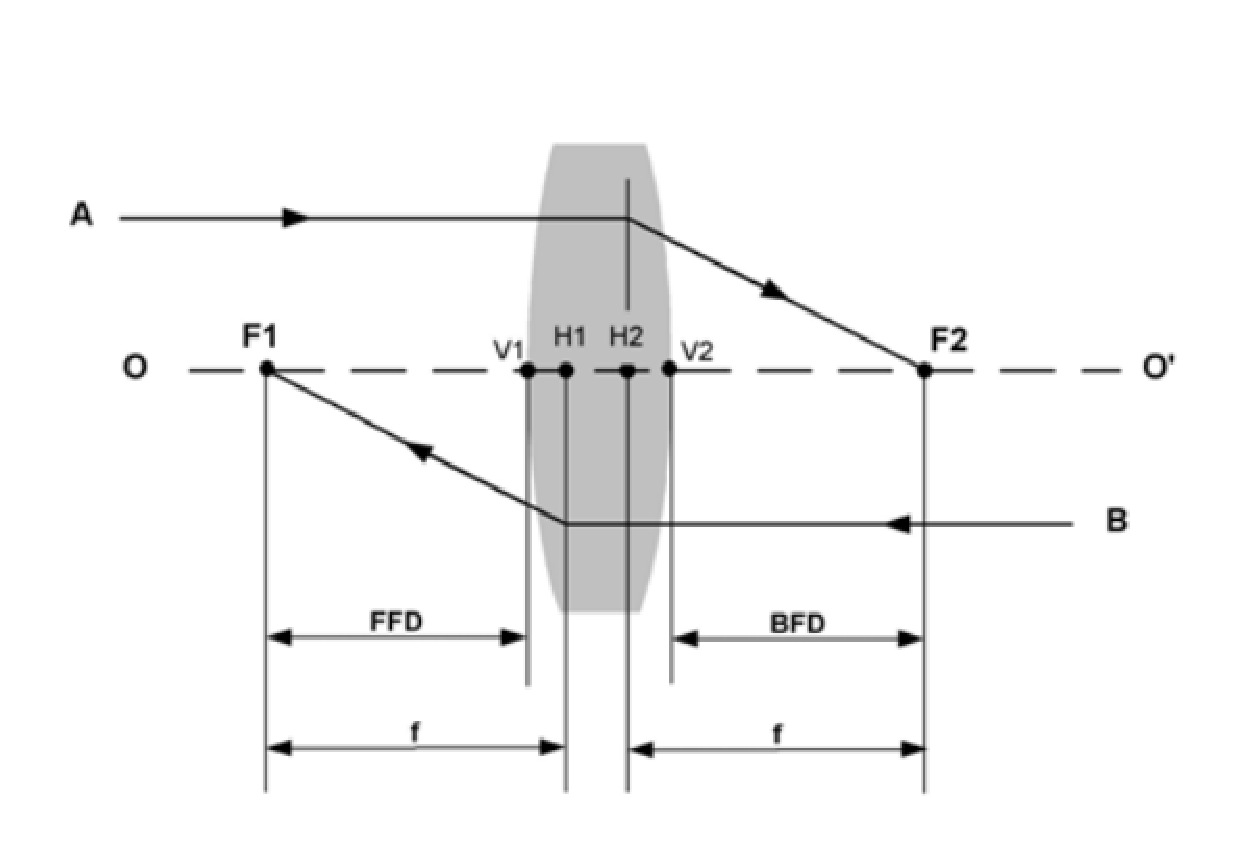
\includegraphics[width=0.6\textwidth]{bilder/lens_define}
\caption{The quantities define of singlet lenses \cite{lens_theory_LC_Ltd}}
\label{fig:lens_define}
\end{figure}
In order to understand more specifics about lenses Fig.\ref{fig:lens_define}  presents a singlet lens with geometric parameters. \"The optical axis (O-O')of the lens is a line passing through the centers of curvature of the two spherical lens surfaces. \"
Rays A and B, parallel with the optic axis (O-O'), are casted from different two sides through the lens and respectively cross the axis at their front and back focal points $F1$ and $F2$. The front and back principal points $H1$ and $H2$ are the intersections of the optical axis with the front and back principal surfaces. Points $V1$ and $V2$ are called the front and back vertices respectively\cite{lens_theory_LC_Ltd}.  Some important quantities are defined in Tab. \ref{tab:lens_quantities}. Here the distance $t_{c}$ is the center thickness of the lens $V1V2$.\\
\begin{table}
\centering
\caption{Important Quantities for Singlet Lenses Immersed in Air\cite{lens_theory_LC_Ltd}.}
\begin{tabular}{|c|c|c|}
\hline
\textbf{Symbol}&\textbf{Description}&\textbf{Formular}\\
\hline
$f$ & \parbox[c]{6cm}{
						\begin{center}
						effective focal length
						\end{center}
				}& $\frac{1}{f}=(n-1)\left[\frac{1}{R_{1}}-\frac{1}{R_{2}} \right]+\frac{t_{c}(n-1)^2}{nR_{1}R_{2}}$ \\
\hline
$BFD$ &\parbox[c]{6cm}{
						\begin{center}
						back focal distance 
						\end{center}
			}& $BFD=f\left[ 1-\frac{t_{c}(n-1)}{nR_{1}}\right]$ \\
\hline
$FFD$ &\parbox[c]{6cm}{
						\begin{center}
						 front focal distance
						 \end{center} 
			}& $FFD=f\left[ 1+\frac{t_{c}(n-1)}{nR_{1}}\right]$ \\
\hline
$H2V2$ & \parbox[c]{6cm}{
						\begin{center}
						back vertex to back principal point distance
						\end{center}						
			} & $H_{2}V_{2}=f-BFD=-f\frac{t_{c}(n-1)}{nR_{1}}$ \\
\hline
$V1H1$ & \parbox[c]{6cm}{
						\begin{center}			
				    front vertex to front principal point distance
				    \end{center}
				 } & $V_{1}H_{1}=f-FFD=-f\frac{t_{c}(n-1)}{nR_{2}}$ \\
\hline
\end{tabular}
\label{tab:lens_quantities}
\end{table}
The classical singlet lenses are plano convex, plano concave, equiconvex and equiconcave lenses, which are listed in following Tab.\ref{tab:lenses_focal_length} with their focal length relation.The performance of a lens is usually estimated by spot size and focal lengths. The definition of the spot size will be declared later in section \ref{sect:gaussian_beam}. The focal length is in common sense the distance from lens center to minimum spot. But this idea is not exact in any case.  Here we can testify this thought by Fig. \ref{fig:focal_length} and following equations (\ref{eq:snell_focal}-\ref{eq:focal_length}).\\
\begin{table}[!ht]
\centering
\caption{Focal length Formulas of Simple Singlet Lenses in Air and  
				 the Radii are considered positive in the formulas below\cite{lens_theory_LC_Ltd}.}
\begin{tabular}{|c|c|c|}
\hline
\textbf{Type}&\textbf{Description}&\textbf{Formula}\\
\hline
Plano Convex & \parbox[c]{2.1cm}{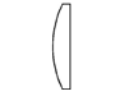
\includegraphics[width=2cm]{bilder/plano_convex}}& $f=\frac{R}{(n-1)}$ \\
\hline
Plano Concave &\parbox[c]{2.1cm}{
\includegraphics[width=2cm]{bilder/plano_concave}} & $f=-\frac{R}{(n-1)}$ \\
\hline
Equiconvex & \parbox[c]{2.1cm}{
\includegraphics[width=2cm]{bilder/equi_convex}} & $f=\left[\frac{2(n-1)}{R} - \frac{t_{c}(n-1)^2}{nR^2}\right]^{-1}$ \\
\hline
Equiconcave & \parbox[c]{2.1cm}{
\includegraphics[width=2cm]{bilder/equi_concave}} & $f=\left[\frac{2(n-1)}{R} + \frac{t_{c}(n-1)^2}{nR^2}\right]^{-1}$ \\
\hline
\end{tabular}
\label{tab:lenses_focal_length}
\end{table}
\begin{figure}[!ht]
\centering
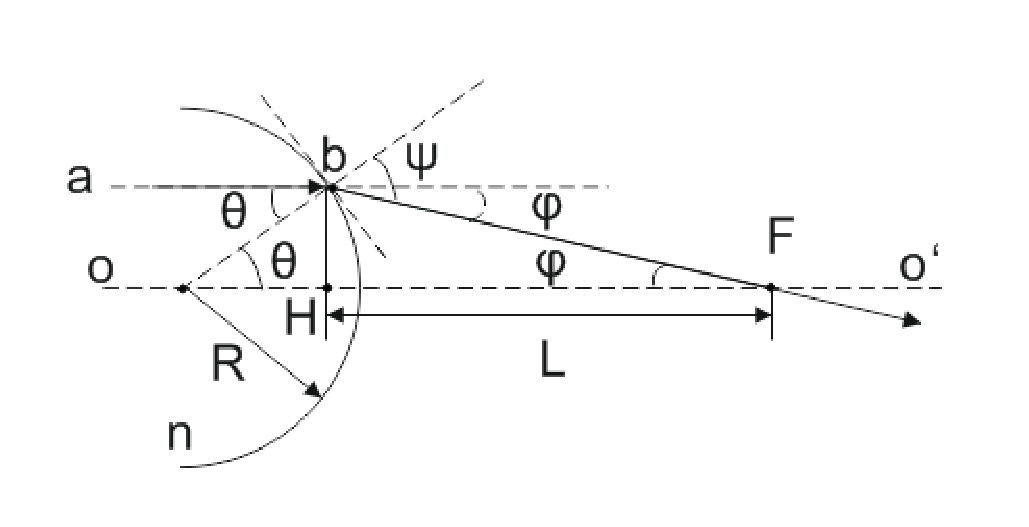
\includegraphics[width=0.6\textwidth]{bilder/focal_length}
\caption{Schema of refraction of parallel light by lens.}
\label{fig:focal_length}
\end{figure}

\begin{equation}
nsin\theta=sin\psi
\label{eq:snell_focal}
\end{equation}
\begin{equation}
\phi=\psi-\theta
\label{eq:psi_phi}
\end{equation}
\begin{align}
L&=Rsin(\theta) ctan(\phi) \nonumber\\
&=Rsin(\theta)\frac{cos(\psi-\theta)}{ sin(\psi-\theta)} \nonumber\\
&= Rsin(\theta)\frac{cos(\psi)cos(\theta)+sin(\psi)sin(\theta)}{sin(\psi)cos(\theta)-cos(\psi)sin(\theta)} \nonumber\\
&= Rsin(\theta)\frac{cos(\psi)cos(\theta)+nsin^{2}(\theta)}{nsin(\theta)cos(\theta)-cos(\psi)sin(\theta)} \nonumber\\
&=R\frac{cos(\psi)cos(\theta)+nsin^{2}(\theta)}{ncos(\theta)-cos(\psi)} \nonumber\\
&=R\frac{cos(\psi)cos(\theta)-ncos^{2}(\theta)+n}{ncos(\theta)-cos(\psi)} \nonumber\\
&=R \left[-cos(\theta)+\frac{n}{ncos(\theta)-\sqrt{1-n^{2}sin^{2}(\theta)}} \right]
\label{eq:focal_length}
\end{align}
In Fig. \ref{fig:focal_length} there is a lens with radius $R$ and index $n$. O-O' axis goes through the lens center.  The light source $a$ emits a ray parallel with the O-O' axis and at the point $b$ on the lens surface is refracted. At last the refracted ray cross the O-O' axis at point F. $\theta$ is the input angle, $\psi$ the output angle and $\phi$ the angle from output ray to O-O' axis. According the SNELL's LAW we get the relation between $\theta$ and $\psi$ in (\ref{eq:snell_focal}). $\phi$ and $\psi$ has the relation like (\ref{eq:psi_phi}). Then the distance $L$ from point H to F is given by (\ref{eq:focal_length}). When $\theta$ is close to 0 like (\ref{eq:focal_length_app}) $L$ is right equal the formula of Plano Convex in Tab. \ref{tab:lenses_focal_length}. So this formula of focal length is only valid for a small angle lens. 
\begin{equation}
L=R\left[ -1+\frac{n}{n-1}\right]=\frac{R}{n-1}
\label{eq:focal_length_app}
\end{equation}
Where is the focal point indeed located? \cite{lens_theory_LC_Ltd} has refered that the minimum spot lies between the maeginal plane and paraxial focal plane. All the distances which are in following discussed base on the assumption that the back vertex (V2) of the lens is regarded as origin. In Fig.\ref{fig:min_max_spot} there are "'geometrical traces of 25 rays in the focal region 100mm focal length plano convex lens(n=1.515)."'  "'The rays are launched parallel to the axis (O-O') and equally spaced in a region above and below the axis in a plane containing the axis(\textbf{meridional plane})"'. The marginal plane (\textbf{MP}) goes through the focal point of marginal rays. The paraxial focal plane (\textbf{PP}) goes through the focal point of paraxial rays. "'The distance from \textbf{PP} to \textbf{MP} is the \textbf{longitudinal aberration LAm}"'. The minimum spot (\textbf{MS}) is located at the plane, which is approximately 3/4 LAm back toward the lens from the \textbf{PP}.
\begin{figure}[httbp]
\centering
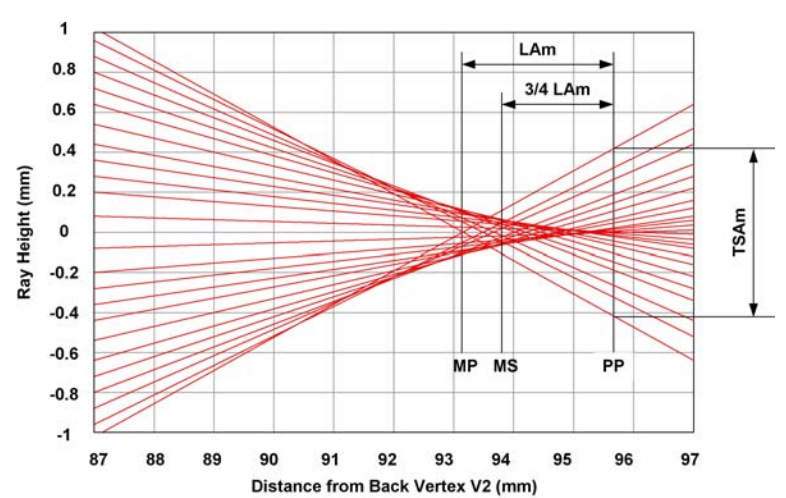
\includegraphics[width=0.9\textwidth]{bilder/min_max_spot}
\caption{Schema to estimating the minimum spot location \cite{lens_theory_LC_Ltd}.}
\label{fig:min_max_spot}
\end{figure}


\subsection{Fiber optics}
Optical fibers are widely used as a medium for telecommuniction and networking because of varity of advantages.It is flexible,especially permits transmission over longer distances and at higher bandwidths (data rates) than other forms of communication. The Fig.\ref{fig:opticfiber} presents a simplest optical fiber and how lights progate in the fiber. 

\begin{figure}[httbp]
\centering
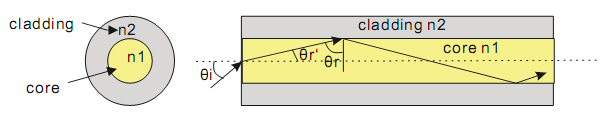
\includegraphics[width=0.8\textwidth]{bilder/opticfiber}
\caption{linght refraction in optic fibers}
\label{fig:opticfiber}
\end{figure}

Optical fiber typically consists of a transparent core with index $n1$ surrounded by a transparent cladding material with a lower index of refraction $n2$. The Light is kept in the core by total internal reflection. This causes the fiber to act as a waveguide.
In \cite{script_FT_TET} the principle of the total reflection is explained with Snell's law. When a light or wave pass through a boundary between two different isotropic media, it behaves after Snell's law, which is presented in following mathematical fomular (\ref{lab:snell}).

\begin{equation}
n_{1}sin\theta_{r}=n_{2}sin\theta_{t}
\label{lab:snell}
\end{equation}



\theta_{t} is transmission angle or refraction angle.